\section{The First ``C'': Cache-conscious \Bv Design} \label{sec:bv-design}

% As discussed in~\secref{intro}, existing state-of-the-art succinct tries
% suffer from poor cache locality of dedicated \bv operations.
In this section, we present the first "C" of \csquared:
\underline{C}ache-conscious bitvector design (denoted with \bvdesign). First,
inspired by prior work\\~\cite{optimized_rank, terark_bv}, we apply an
array-of-structs reorganization to bitvectors to better exploit the access
pattern of \rankop queries. Second, we eliminate cache misses from reading the
\selectop index using our novel \emph{functional index}. Third, to handle both
sparse and dense patterns, \rev{we further optimize the existing technique of
  overflowing \selectop indexes and reduce cache misses by storing all data
  in-place}. Finally, we apply the above techniques to three state-of-the-art
\mymarginpar{Meta 4}\rev{LOUDS-based} succinct tries~\cite{surf, coco_0,
  marisa}.

\rev{We adopt two design principles: (1) optimization priority of
  cache $>$ branch $>$ arithmetic operations~\cite{rank_select_1}, and (2)
  trading space for performance. Since trie topologies are usually much smaller
  than trie labels, a small space overhead is worthwhile for increased query
  speed.}

\para{Locality issues in \bvs} \newmymarginpar{Meta 1, R1 O2}\newrev{The main
  challenge to locality during trie navigation arises from storing the index and
  \bv separately~\cite{rank_select_0, rank_select_1, rank_select_2,
    rank_select_3, sds_overview, ds2i, surf}, since both must be accessed during
  \rankop and \selectop. Packing the \rankop index with the bit sequence
  improves locality for \rankop~\cite{optimized_rank, terark_bv}, but the same
  approach does not work for \selectop. In most cases, the input to \rankop maps
  linearly to a position in the bit sequence; \newmymarginpar{R2 O3/D6}the input
  to \selectop, however, is often an intermediate value (e.g.\ the output of
  \rankop) with no straightforward mapping to a bit position.}
  %This indirection prevents packing the \selectop index with the bit sequence.}

\begin{figure}[t]
    \centering
    \begin{minipage}[h]{.19\textwidth}
    \includegraphics[width=\textwidth,page=5,trim=13cm 6.5cm 14cm 6cm,clip]{visualization.pdf}
        \caption{Interleaving.}
        \label{fig:interleaving}
    \end{minipage}
    \hspace{0.1cm}
    \begin{minipage}[h]{.26\textwidth}
        \includegraphics[width=\textwidth,page=7,trim=12cm 5cm 10cm 6cm,clip]{visualization.pdf}
        \caption{Select index overflow.}
        \label{fig:overflow}
    \end{minipage}
\end{figure}

\subsection{Array-of-Struct Reordering}\label{sec:interleaving}

Most traditional \bvs are organized in a struct-of-array manner. During \rankop
queries, each query accesses the target block immediately after its \rankop
index. To better exploit this locality, \rankop indexes can be \mymarginpar{Meta
  5, R2 D13}\rev{\defn{interleaved}, or stored in an array-of-structs manner
  with the index and bitvector in one contiguous memory allocation, as
  illustrated in \figref{interleaving}.}
  %Storing the rank index interleaved with
  %its associated blocks reduces cache misses \cite{optimized_rank, terark_bv}.}

Similarly, for tries encoded with multiple \bvs, we interleave blocks of
different \bvs that are often jointly accessed at nearby bit positions. For
example, in LOUDS-Sparse, we pack the blocks of \haschild and \louds, as they
are aligned with each other and are typically accessed together. \rev{Similarly,
  we can interleave secondary \rankop indexes~\cite{optimized_rank,
    terark_bv, sds_overview, rank_select_3, marisa}.} %, if the trie uses them.}

We restrict the size of each \rankop index \rev{element} to 32 bits \rev{for
  better space efficiency without loss of applicability to larger datasets}. To
support \bvs larger than $2^{32}$ bits, previous work shows how to first
\emph{partition} the data into \rev{connected} sub-tries that individually fit
in the size limit~\cite{hybrid_surf}.

\subsection{Functional Index}\label{sec:functional-index}
% \helen{is it correct that the most novelty is in here?}
  \begin{figure}[t]
    \centering
    \includegraphics[width=\columnwidth,page=13,trim=3cm 8.4cm 8cm 3.5cm,clip]{visualization.pdf}
    \caption{ \rev{Functional index example for LOUDS-Sparse's \texttt{Child(x)
          = Louds.select}$_1$\texttt{(HasChild.rank}$_1$\texttt{(x + 1) +
          1)}. The block size and the sampling rate for \selectop (left) are
        both 5. The third row on the right (\texttt{Child}) caches the results
        of \texttt{Child(x)} at the start of block (i.e. \texttt{Child(0)},
        \texttt{Child(5), etc.}).}}
    \label{fig:functional-index}
\end{figure}

To improve spatial locality for \selectop, we introduce the \defn{functional
  index} \mymarginpar{R2 D14}\rev{that samples results of the navigation
  function (e.g., \texttt{Child(x)}) rather than intermediate \selectop values.}
For example, to support child navigation in LOUDS (where
$\texttt{Child(x)} =
\selectopnospace_0\texttt{(}\rankopnospace_1\texttt{(x+1))+1}$), we sample
\texttt{Child(x)}, instead of \\$\selectopnospace_0$\texttt{(x)}, at regular intervals of
$x$. Since the sampled function is monotonically non-decreasing, the sampling is
unambiguous. \rev{We then interleave these samples with blocks for spatial
  locality.} Other succinct trie operations (e.g., parent navigation) can be
optimized using similar approaches.

\mymarginpar{R1 D2}\new{\figref{functional-index} shows a worked example of
  computing \texttt{Child(6)} using traditional and functional indexes. An
  implementation using the traditional index first computes
  \texttt{HasChild.\rankopnospace$_1$(6+1)=7} (by accessing \texttt{HasChild}'s
  rank index and the \texttt{HasChild} bitvector) and then obtains
  \texttt{Louds.select$_1$(7+1)=13} (by accessing \texttt{Louds}' select index
  and the \texttt{Louds} bitvector itself), which easily incurs 4 cache
  misses. In contrast, using the cache-optimized functional index, we first
  access block 1 (which bit 6 falls into) and obtain
  \texttt{HasChild}.\rankopnospace$_1$(6+1) = 7 (using block 1's rank
  index). Then, we read block 1's functional index for \texttt{Child}, which
  stores the value of \texttt{Louds}.\selectopnospace$_1$(5+1) = 9. Since we
  need to compute \selectopnospace$_1$(7+1), we select two more ones starting
  from bit 9 and end up at bit position 13.

   Assuming the two accessed blocks belong to different cache lines, we incur
   only two cache misses in total.} \rev{In practice, since} trie navigation
 operations are often executed in a pipelined manner (\textit{i.e.}, the output
 of one operation is immediately used as the input \rev{of} the next operation),
 this optimization essentially cuts cache misses by $4\times$ in long pipelines.

 \newrev{\para{Applicability beyond LOUDS}
   Although we develop and evaluate the functional index in the context of
   LOUDS-based tries, the core idea applies to any succinct-tree encoding whose
   navigation functions are monotonically non-decreasing compositions of \rankop
   and \selectop. The key insight behind the functional index is that
   \texttt{Child(x)} is a function of the position \texttt{x}, not of an
   intermediate bitvector value, so sampling it at regular intervals of
   \texttt{x} aligns the index with the bit sequence and enables
   interleaving. This property holds in BP and DFUDS as well, since the
   navigation function's input and output both increase monotonically with the
   traversal order of the encoding.

\newmymarginpar{R2 O4/D7, R3 O3/D3}
  In BP, child navigation reduces to a \texttt{findclose} operation (i.e.,
  locating the matching close parens for an open parens),% at position \texttt{x}),
  which is implemented via \rankop/\selectop on the parenthesis \bv. The
  functional index directly applies because \texttt{findclose(x)} is
  monotonically non-decreasing in \texttt{x}, so it can be directly sampled at
  regular intervals of \texttt{x} and interleaved with the bit
  blocks. Similarly, DFUDS navigation starts with the \texttt{Child(x, 1)}
  operation, which returns the first child of the node at position
  \texttt{x}. This first-child operation admits a functional index in
  the standard way, with subsequent siblings located by scanning forward.
  %— a
  %pattern that is efficient in practice because node fanouts are typically
  %small.
  % The PDT [22], which is DFUDS-encoded, is thus a natural candidate for the
  % functional index: it already incurs significant bitvector overhead during
  % navigation, and our analysis of BP and DFUDS in Section 2.2 suggests that
  % the same cache-miss reduction achieved in LOUDS-based tries would apply
  % there. We leave a full evaluation of the functional index under BP and DFUDS
  % to future work, noting it as a direct extension of the C1 optimization
  % described here.
}


\subsection{Overflow of Select Index}\label{sec:overflow}

So far, we have assumed that the probe distance within the target interval is
small. But this is not always the case, especially for the CoCo-trie, which
sometimes contains nodes with very large fan-outs. For instance, when encoding
the \texttt{trec-terms}~\cite{trec_dataset} dataset in the original CoCo-trie
paper, the first 600k bits of the CoCo-trie topology contain only 36
\rev{zero}\mymarginpar{Meta 5, R2 D17} bits. With such extreme sparsity, regular
searching algorithms would be too slow.

A classic solution to this problem is to allow the \selectop index to overflow
\cite{ds2i, rank_select_3}. That is, the \selectop index should detect regions
with extremely low pattern density, and precompute every \selectop result in
those regions. Since the precomputed results do not fit in regular sample space,
they are overflowed to a separate list, and the sample stores a pointer to the
overflow list instead.

\rev{Unfortunately, overflowing the select index disrupts locality because two
  adjacent samples\mymarginpar{R2 D16} are no longer guaranteed to form a
  bounding interval, as either of them can be overflowed. Therefore,} after
querying the sample, we must either use linear search or incur an additional
cache miss to read the spill list.

We resolve this issue by storing \emph{block indexes} instead of exact bit
positions in regular samples, as this frees up additional bits to store the size
of the bounding interval \rev{(in blocks)}. The \rankop indexes in each block
provide enough information to restore any lost precision at no cost of
additional cache misses. \new{For example, in \figref{functional-index}, block
  1's functional index for \texttt{Child} (i.e. \texttt{Child(5)}) points to
  block 1, which is equivalent to bit position 5 (instead of its original value
  9 in~\figref{functional-index}). Using the inlined rank index, we immediately
  restore \texttt{HasChild.\rankopnospace$_1$(5) = 5}. Since \texttt{Child(5) =
    Louds.\selectopnospace$_1$(7)}, we can reach position \texttt{Child(5)}
  (i.e., 9) by selecting two more ones.}

As shown in \figref{overflow}, each sample occupies 32 bits, where bit 31
indicates whether the sample overflows. If bit 31 is false, then bits 7 to
30 (the 24-bit \head, which means block size must be at least 256) point to the
lower bounding block, whereas bits 0 to 6 (the 7-bit \dist) \rev{store the
  length of the bounding interval (in blocks).}  If \dist does not fit in 7 bits
(\textit{i.e.}, the bounding interval is at least 128 blocks long), then bit 31
is set to true, and the sample is overflowed. The rest of the sample (the 31-bit
\spillptr) \rev{indexes} into the centralized overflow list \spilllist, where
\texttt{\spilllistnospace[\spillptr + i]} is the position of the $i$-th target pattern
in the overflowing interval. \rev{We apply this optimization to} both traditional \selectop indexes and functional indexes with intermediate selects.

We sketch why \spillptr always fits in 31 bits. With block size $B=256$ and
sample rate $S=256$, each overflowing interval has target pattern density at
most $S/128B = 1/128$ (for \selectop indexes) or $B/128B = 1/128$ (for
functional indexes). Since the \bv size does not exceed $2^{32}$, the size of
\spilllist would not exceed $2^{32}/128 = 2^{25}$ and hence \rev{always fits} in
26 bits.

\mymarginpar{R3 O1}\new{Finally, we address the space overhead incurred by the
  spill list. Because each spilled interval contains at most $B = 256$ bits, the
  density of ones is at least 256/(256$ \times$ 128) = 1/128, and the associated
  spill list occupies at most 32/128 = 25\% of the bitvector size. For
  LOUDS-encoded tries, since only half of the bits are zeros, the bound can be
  reduced to 25\% $\times$ 128/127/2 = 12.6\%. For LOUDS-Sparse encoded tries,
  the functional index is sampled on only one of the two bitvectors, which also
  tightens the bound to 12.5\%. Both upper bounds are reached only under extreme
  conditions where most trie edges are concentrated in a few large nodes, which
  is unlikely in practical datasets.}

\subsection{Applying the Rules}

\begin{figure}[t]
    \centering
    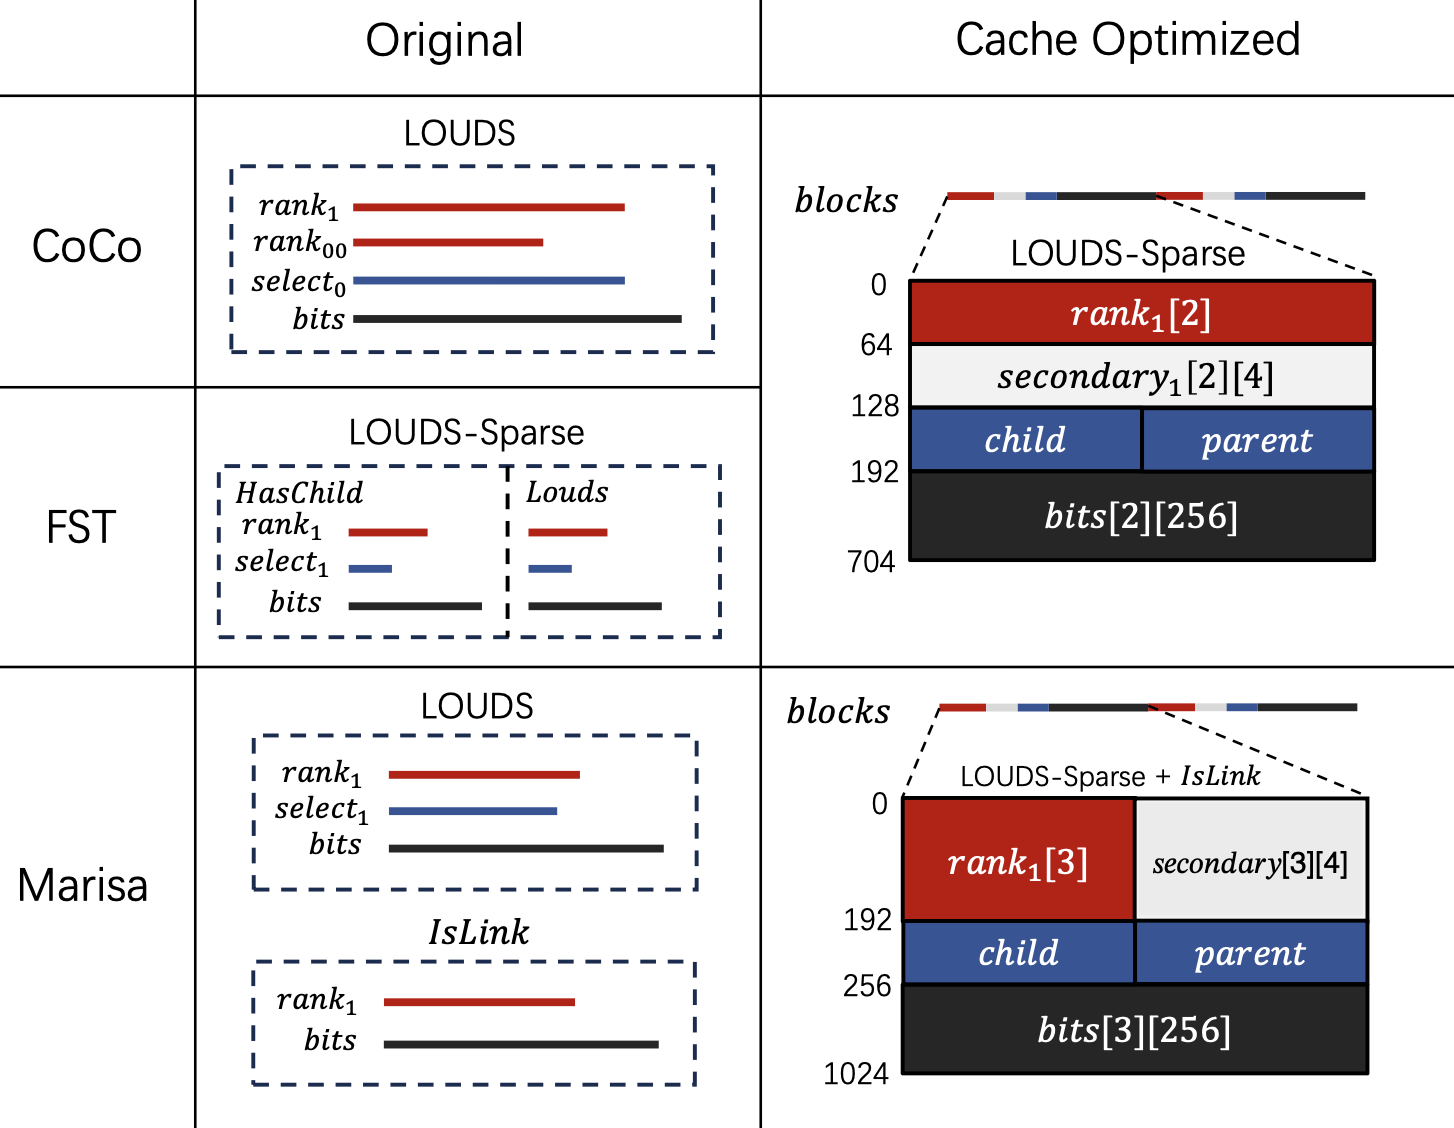
\includegraphics[width=\columnwidth]{bv-figure}
    \caption{Optimized \bv layout. \rev{\child: functional index for
        \var{Child(x)}. \parent: functional index for
        \var{Parent(x)}. \texttt{secondary}$_1$: secondary index for
        \rankopnospace$_1$.  }}
    \label{fig:bv-design}
  \end{figure}
\iffalse
\begin{figure}[t]
    \centering
    \includegraphics[width=\columnwidth,page=8,trim=0cm 3.6cm 14cm 0cm,clip]{visualization.pdf}
    \caption{Optimized \bv layout. \rev{\child: functional index for
        \var{Child(x)}. \parent: functional index for
        \var{Parent(x)}. \texttt{secondary}$_1$: secondary index for
        \rankopnospace$_1$.  }}
    \label{fig:bv-design}
  \end{figure}
  \fi

We apply the above optimizations to FST, CoCo-trie, and Marisa;
\figref{bv-design} shows the resulting \bv layouts.

The FST is encoded using LOUDS-Sparse and only needs to support existence
query. We pack the blocks of \haschild and \louds (\secref{interleaving}) and
interleave bits with the \rankopnospace$_1$ (\secref{interleaving}) and \child
(\secreftwo{functional-index}{overflow}) indexes.

%\todo{update this part to move coco to louds sparse?}
\rev{The CoCo-trie is encoded using standard LOUDS and supports top-down lookup,
  and therefore an ideal approach is to inline (primary and secondary)
  \rankopnospace$_1$ and \rankopnospace$_{00}$ indexes (\secref{interleaving})
  and the \child (\secref{functional-index}, \secref{overflow}) functional
  index. However, this adds a 192-bit space overhead to every 256-bit block,
  which is too expensive. Therefore, we switch to LOUDS-Sparse encoding which
  incurs less index overhead.}

The case with Marisa is \rev{more}\mymarginpar{R2 D15} involved. First, we
change the encoding scheme from LOUDS to LOUDS-Sparse, as this allows for better
alignment. Then, we pack the blocks of \haschild, \louds and \islink, as all
three \bvs are now edge-aligned and are typically accessed with high locality
(\secref{interleaving}). Finally, we interleave the bits with indexes for \child
and \parent(\secref{functional-index}, \secref{overflow}), and each \bv's
\proc{rank}$_1$ (\secref{interleaving}) indexes, as the Marisa trie needs to
support both \rev{forward and reverse lookups}. %(i.e. reverse) lookups.

\new{\para{Theoretical analysis} The $C_1$ optimizations preserve asymptotic
  bounds on space and query complexity. The rank and select indexes are
  lower-order terms relative to the bitvector size~\cite{surf}. \mymarginpar{R1 W2, R1 D4}}

\new{\begin{lemma} Given a \bv of size $S$ and a block size of $B$, the $C_1$ optimizations incur at most $S/2B$ additional space overhead.
%compared to the original LOUDS-Sparse.
\end{lemma}

\begin{proof}
  % A trie with $n$ nodes takes about $10n$ bits to encode in LOUDS-Sparse,
  % which is close to the information-theoretic lower bound of about $9.44n$
  % bits~\cite{surf}. LOUDS-Sparse takes $8n$ bits for the labels and $n$ bits
  % each for the Louds and Has-Child \bvs (see~\secref{preliminaries}).
  The size of the rank index in $C_1$ is unchanged and takes 32 bits per
  block. %, for an overhead of 12.5\% when $B = 256$.
  Since only half of the bits in a trie encoding are 1, the \selectopnospace$_1$
  index contains about $S/2B$ elements, whereas the \texttt{Child} functional
  index contains $S/B$ elements.
\end{proof}
} \rev{Although functional indexes use more space compared to traditional
  \selectop indexes,\mymarginpar{R2 D16} the overall space overhead is small
  relative to the index size and label data. For example, when $B=256$, the
  functional index takes 12.5\% extra space relative to the \bv size compared to
  the \selectop index.}

% Furthermore, as mentioned earlier, the $C_1$ optimization reduces the cache
% misses during child navigations.

\begin{lemma}
  A child navigation takes at most 4 cache misses in all of the
  \bvdesign-optimized tries in this paper.
\end{lemma}

\begin{proof}
  Let \bvdesign-CoCo, \bvdesign-FST, and \bvdesign-Marisa denote the CoCo-trie,
  FST, and Marisa trie with the $C_1$ optimization as illustrated
  in~\figref{bv-design}.  As shown in~\figref{bv-design}, \bvdesign-CoCo,
  \bvdesign-FST, and \bvdesign-Marisa have block sizes of 704, 704, and 1024
  bits, respectively. Given a cache-line size of 64 bytes (512 bits), each block
  in the \bvdesign-optimized succinct tries takes at most 2 cache lines.  A
  child navigation with the functional index queries two blocks: the input block
  and the output
  block. %, for at most 2 cache misses in the \bvdesign-CoCo, and at most 4
         %cache misses in the FST and Marisa trie with $C_1$.
\end{proof}

Although the blocks in the \bvdesign-optimized tries span 2 cache lines each,
the second cache line in the block is prefetched and therefore incurs no
additional cache misses. In contrast, the original succinct tries (e.g., CoCo,
FST, and Marisa), are encoded using separate \bvs, which take at least 3 random
cache misses per block.

%%% Local Variables:
%%% mode: latex
%%% TeX-master: "main"
%%% End:
